\documentclass[12pt]{article}
%\usepackage[utf8]{inputenc}
%\documentclass[UTF8]{ctexart}
%\usepackage[UTF8, heading = false, scheme = plain]{ctex}
\usepackage{geometry}
%geometry{a4paper,scale=0.9}
\geometry{a4paper,left=1cm,right=1cm,top=1cm,bottom=2cm}
\usepackage{amsfonts}
\usepackage{color}
\usepackage{url}
%\usepackage{biblatex}
\usepackage{amsmath}
\usepackage{amssymb}
\usepackage{latexsym}
\usepackage[linesnumbered,ruled,lined]{algorithm2e}
\usepackage{pythonhighlight}
\usepackage{listings}
\usepackage{cite}
%\addbibresource{ref.bib}
%\bibliography{ref.bib}
\usepackage{caption}
\usepackage{graphicx, subfig}
\usepackage{float}
%\usepackage[fontset=ubuntu]{ctex}
%\usepackage{fontspec}
\usepackage{xeCJK}
%\usepackage[colorlinks,
%anchorcolor=black,
%citecolor=black]{hyperref}
%\setmainfont{SimSun}
\usepackage[section]{placeins}
\usepackage{enumitem}
\usepackage{framed}
\usepackage[framemethod=TikZ]{mdframed}
\usepackage{indentfirst}
\usepackage{setspace}%使用间距宏包
\linespread{1.5}

\lstset{
keywordstyle=\color{blue!70}\bfseries, %设置关键词为蓝色,需要引xcolor宏包,
basicstyle=\ttfamily, 
commentstyle=\ttfamily, %基本和注释的字体都使用默认的等宽,而非texlive调用的中文字体
%commentstyle=\color{red!50!green!50!blue!50},
showstringspaces=false, %不显示中间的空格
frame=shadowbox,  %边框
breaklines,%自动换行
columns=flexible,%不随便添加空格,只在已经有空格的地方添加空格,
%如果想要添加空格使用fixed作为参数(这是默认的),如果坚决不添加空格使用fullflexible作为参数.
frame=shadowbox, 
rulesepcolor=\color{red!20!green!20!blue!20}
}

\title{TensorFlow\cite{TensorFlow_Tutorial_From_Zero_1}\cite{TensorFlow_Tutorial_Official}\cite{TensorFlow_Tutorial_Quick_Detailed}}
\author{leolinuxer}
%\date{June 2020}

\begin{document}
%\setlength{\parindent}{0pt}
\maketitle
\tableofcontents

\section{安装Tensorflow}
\subsection{通过 conda 手动安装总结}
1. 安装 minconda

2. 修改 conda 国内镜像

3. 安装相关依赖(不知道是不是必须的步骤)(github上搜索Jeff heaton,找到 t81\_558\_deep\_learning仓库,划到最下方找到tensorflow.yml 可以查看 tensorflow的依赖 )
\begin{lstlisting}
pip install bayesian-optimization gym kaggle
\end{lstlisting}

4. 安装 tensorflow:
\begin{lstlisting}
conda create -n tf #新建conda环
conda activate tf #激活conda环境
conda install jupyter
conda install python=3.6
conda install tensorflow=2.0
\end{lstlisting}

5. 检查TensorFlow的命令行
\begin{lstlisting}
python
import tensorflow as tf
print(tf.__version__)
#输出结果应该为2.0.0
\end{lstlisting}

\subsection{通过 conda 安装}
\subsubsection{下载并安装 minconda}
下载地址:\url{https://links.jianshu.com/go?to=https%3A%2F%2Fdocs.conda.io%2Fen%2Flatest%2Fminiconda.html}

安装成功后重启 Mac 生效

\subsubsection{下载环境安装脚本}
github上搜索Jeff heaton,找到 t81\_558\_deep\_learning仓库,划到最下方找到tensorflow.yml,用浏览器打开后点击保存在你用户名的文件夹下。

下载地址:\url{https://links.jianshu.com/go?to=https%3A%2F%2Fgithub.com%2Fjeffheaton%2Ft81_558_deep_learning}

\subsubsection{conda国内镜像修改}
来源:\url{https://zhuanlan.zhihu.com/p/95100538}

在使用安装conda 安装某些包会出现慢或安装失败问题,最有效方法是修改镜像源为国内镜像源。之前都选用清华镜像源,但是2019年后已停止服务。推荐选用中科大镜像源。


\begin{lstlisting}
#先查看已经安装过的镜像源,cmd窗口执行命令:
conda config --show
#查看配置项channels,如果显示带有tsinghua,则说明已安装过清华镜像。
#下一步,使用conda config --remove channels url地址删除清华镜像,如下命令删除第一个。然后,依次删除所有镜像源
conda config --remove channels https://mirrors.tuna.tsinghua.edu.cn/tensorflow/linux/cpu/

#添加目前可用的中科大镜像源:
conda config --add channels https://mirrors.ustc.edu.cn/anaconda/pkgs/free/
#并设置搜索时显示通道地址:
conda config --set show_channel_urls yes
#确认是否安装镜像源成功,执行conda config --show,找到channels值为如下:
channels:
  - https://mirrors.ustc.edu.cn/anaconda/pkgs/free/
  - defaults
#安装成功
\end{lstlisting}

\subsubsection{通过conda安装Jupyter}
terminal里输入:
\begin{lstlisting}
conda install jupyter
\end{lstlisting}

\subsubsection{创建环境}
terminal里输入:
\begin{lstlisting}
conda env create -v -f tensorflow.yml

#如果出现如下错误:
conda.exceptions.ResolvePackageNotFound:
  - bayesian-optimization
  - gym
  - kaggle
#则通过 pip 安装上面三个包:
pip install bayesian-optimization gym kaggle
# tensorflow.yml 里面也声明了这三个依赖,不知道为什么没有自动生效

####### 仍然安装失败,尝试手动安装:
conda create -n tf 	#新建conda环
conda activate tf	#激活conda环境
conda install python=3.6	#安装依赖的 python 包
conda install tensorflow	#安装 tensorflow
\end{lstlisting}

\subsubsection{检查TensorFlow的命令行}
terminal里依次输入:
\begin{lstlisting}
conda activate tensorflow
python
import tensorflow as tf
print(tf.__version__)
#输出结果应该为2.0.0
\end{lstlisting}

\subsubsection{conda常见命令}
\begin{lstlisting}
1. conda --version #查看conda版本,验证是否安装
2. conda update conda #更新至最新版本,也会更新其它相关包
3. conda update --all #更新所有包
4. conda update package_name #更新指定的包
5. conda create -n env_name package_name #创建名为env_name的新环境,并在该环境下安装名为package_name 的包,可以指定新环境的版本号,例如:conda create -n python2 python=python2.7 numpy pandas,创建了python2环境,python版本为2.7,同时还安装了numpy pandas包
6. source activate env_name #切换至env_name环境
7. source deactivate #退出环境
8. conda info -e #显示所有已经创建的环境
9. conda create --name new_env_name --clone old_env_name #复制old_env_name为new_env_name
10. conda remove --name env_name –all #删除环境
11. conda list #查看所有已经安装的包
12. conda install package_name #在当前环境中安装包
13. conda install --name env_name package_name #在指定环境中安装包
14. conda remove -- name env_name package #删除指定环境中的包
15. conda remove package #删除当前环境中的包
16. conda create -n tensorflow_env tensorflow
conda activate tensorflow_env #conda 安装tensorflow的CPU版本
17. conda create -n tensorflow_gpuenv tensorflow-gpu
conda activate tensorflow_gpuenv #conda安装tensorflow的GPU版本
18. conda env remove -n env_name #采用第10条的方法删除环境失败时,可采用这种方法
\end{lstlisting}


\subsection{通过 pyenv 安装}
\subsubsection{安装前置环境}
以 Mac 环境为例:
\begin{itemize}
\setlength{\itemsep}{0pt}
\setlength{\parsep}{0pt}
\setlength{\parskip}{0pt}
    \item 安装Homebrew
    
\begin{lstlisting}
/usr/bin/ruby -e "$(curl -fsSL https://raw.githubusercontent.com/Homebrew/install/master/install)"
\end{lstlisting}

    \item 安装pyenv
 
\begin{lstlisting}
brew update
brew install openssl
brew install openssl-devel
brew install pyenv
\end{lstlisting}
   
    \item 在.bash\_profile添加环境变量;让环境变量生效
  
\begin{lstlisting}
export PYENV_ROOT=/usr/local/var/pyenv
if which pyenv > /dev/null; then eval "$(pyenv init -)"; fi
source .bash_profile
\end{lstlisting}
  
    \item 安装3.X版本python
    
\begin{lstlisting}
pyenv install 3.5.1

#直接使用pyenv install命令安装Python时,默认从python.org下载指定版本,会非常的慢。
#可以先从搜狐提供的镜像网站下载指定的Python版本到~/.pyenv/cache目录下
wget http://mirrors.sohu.com/python/3.5.2/Python-3.5.2.tar.xz  -P ~/.pyenv/cache

#到下载地址执行 python -m http.server
export PYTHON_BUILD_MIRROR_URL="http://127.0.0.1:8000/"

#执行 pyenv install 3.5.1 会发现,还是从官网下载。不过此时查看http.server上有一条HEAD请求日志,发现不是直接请问的文件名,而是一个64位的字符,将下载的文件名修改成那64位字符。再执行即可:
mv Python-3.5.1.tar.xz c6d57c0c366d9060ab6c0cdf889ebf3d92711d466cc0119c441dbf2746f725c9
python -m http.server
pyenv install 3.5.1

#安装过程中如果出现错误:ERROR: The Python ssl extension was not compiled. Missing the OpenSSL lib?
#注意如下是一行命令
CFLAGS="-I$(brew --prefix openssl)/include" \
LDFLAGS="-L$(brew --prefix openssl)/lib" \
pyenv install -v 3.5.1

#安装过程中出现任何问题,都可以查看官方文档:https://github.com/pyenv/pyenv/wiki/Common-build-problems
\end{lstlisting}

    \item 安装完成后进行更新
\begin{lstlisting}
pyenv rehash
\end{lstlisting}
    
    \item 查看已安装版本

\begin{lstlisting}
//号表示系统当前正在使用的版本
pyenv versions
\end{lstlisting}
    
    \item 切换python版本;并确认 python 版本
    
\begin{lstlisting}
pyenv global 3.5.1
python
\end{lstlisting}
\end{itemize}

\subsubsection{pyenv简介}
pyenv 帮助我们完美的隔离环境,让多个版本的 python 没有任何冲突,完美共存。

\subsubsection{pyenv 常用命令}

\begin{lstlisting}
pyenv install --list # 列出可安装版本
pyenv install <version> # 安装对应版本
pyenv install -v <version> # 安装对应版本,若发生错误,可以显示详细的错误信息
pyenv versions # 显示当前使用的python版本
pyenv which python # 显示当前python安装路径
pyenv global <version> # 设置默认Python版本
pyenv local <version> # 当前路径创建一个.python-version, 以后进入这个目录自动切换为该版本
pyenv shell <version> # 当前shell的session中启用某版本,优先级高于global 及 local
\end{lstlisting}

\subsubsection{使用virtualenv}

\begin{lstlisting}
pyenv virtualenv env # 从默认版本创建虚拟环境
pyenv virtualenv 3.6.4 env-3.6.4 # 创建3.6.4版本的虚拟环境
pyenv activate env-3.6.4 # 激活 env-3.6.4 这个虚拟环境
pyenv deactivate # 停用当前的虚拟环境

# 自动激活
# 使用pyenv local 虚拟环境名
# 会把`虚拟环境名`写入当前目录的.python-version文件中
# 关闭自动激活 -> pyenv local --unset
# 启动自动激活 -> pyenv local env-3.6.4
pyenv local env-3.6.4

pyenv uninstall env-3.6.4 # 删除 env-3.6.4 这个虚拟环境
\end{lstlisting}

\subsubsection{通过 pyenv 安装并使用 python 3.6.6}

\begin{lstlisting}
pyenv install 3.6.6

//创建一个虚拟环境
pyenv virtualenv 3.6.6 my-env

//激活虚拟环境
pyenv activate my-env

//你会发现,在你的终端里面,多了一个类似于 (my-env) 这样的一个东西,这时候你如果执行就是 python 3.6.6 了
python --version

//如果你执行如下命令,它会告诉你 pip 包安装的绝对路径,也是 pyenv 安装目录下的某个文件夹
pip --version
\end{lstlisting}

\subsubsection{安装 TensorFlow}
\begin{lstlisting}
pip install tensorflow
\end{lstlisting}

\section{TensorFlow 相关概念}
\subsection{计算图}
资料来源:\url{http://c.biancheng.net/view/1883.html}

计算图是包含节点和边的网络。本节定义所有要使用的数据,也就是张量(tensor)对象(常量、变量和占位符),同时定义要执行的所有计算,即运算操作对象(Operation Object,简称 OP)。

每个节点可以有零个或多个输入,但只有一个输出。网络中的节点表示对象(张量和运算操作),边表示运算操作之间流动的张量。计算图定义神经网络的蓝图,但其中的张量还没有相关的数值。

为了构建计算图,需要定义所有要执行的常量、变量和运算操作。

\begin{framed}
通过以下步骤定义一个计算图:

在此以两个向量相加为例给出计算图。假设有两个向量 $v_1$ 和 $v_2$ 将作为输入提供给 Add 操作。建立的计算图如下:
\begin{figure}[H]
    \centering
    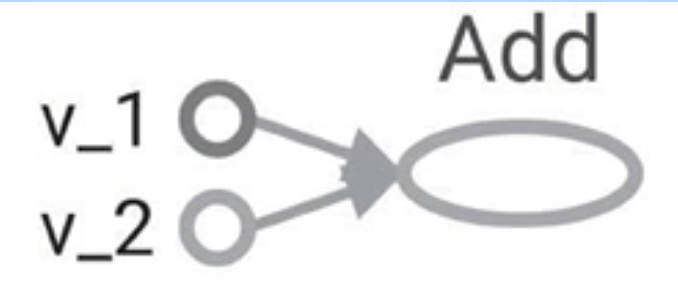
\includegraphics[width=.2\textwidth]{fig/TF_Computational_Graph_Example_Add.png}
\end{figure}

\begin{python}
# 定义该图的相应代码如下所示:
v_1 = tf.constant([1,2,3,4])
v_2 = tf.constant([2,1,5,3])
v_add = tf.add(v_1, v_2) # or v_add = v_1 + v_2

# 在会话中执行这个图:
with tf.Session() as sess:
	print(sess.run(v_add))
	
# 以上两行相当于下面的代码。上面的代码的优点是不必显式写出关闭会话的命令:
# 请记住,每个会话都需要使用 close() 来明确关闭,而 with 格式可以在运行结束时隐式关闭会话。
sess = tf.Session()
print(sess.run(v_add))
sess.close()

## 运行结果是显示两个向量的和:
## {3 3 8 7}
\end{python}
\end{framed}

可以看出,计算图的构建非常简单。添加变量和操作,并按照逐层建立神经网络的顺序传递它们(让张量流动)。TensorFlow 还允许使用 with tf.device() 命令来使用具有不同计算图形对象的特定设备(CPU/GPU)。在例子中,计算图由三个节点组成, $v_1$ 和 $v_2$ 表示这两个向量,Add 是要对它们执行的操作。

\subsection{基础数据类型}
来源:\url{http://c.biancheng.net/view/1885.html}
\subsubsection{基础概念}
张量,可理解为一个 n 维矩阵,所有类型的数据,包括标量、矢量和矩阵等都是特殊类型的张量。

TensorFlow 支持以下三种类型的张量:
\begin{itemize}
\setlength{\itemsep}{0pt}
\setlength{\parsep}{0pt}
\setlength{\parskip}{0pt}
    \item 常量:常量是其值不能改变的张量;
    \item 变量:当一个量在会话中的值需要更新时,使用变量来表示。例如,在神经网络中,权重需要在训练期间更新,可以通过将权重声明为变量来实现。变量在使用前需要被显示初始化。另外需要注意的是,常量存储在计算图的定义中,每次加载图时都会加载相关变量。换句话说,它们是占用内存的。另一方面,变量又是分开存储的。它们可以存储在参数服务器上;
    \item 占位符:用于将值输入 TensorFlow 图中。它们可以和 feed\_dict 一起使用来输入数据。在训练神经网络时,它们通常用于提供新的训练样本。在会话中运行计算图时,可以为占位符赋值。这样在构建一个计算图时不需要真正地输入数据。需要注意的是,占位符不包含任何数据,因此不需要初始化它们。
\end{itemize}

\subsubsection{TensorFlow 常量}
\begin{python}
t_1 = tf.constant(4) #声明一个标量常量
t_2 = tf.constant([4,3,2]) #一个形如 [1,3] 的常量向量
tf.zeros([M,N],tf.dtype) #要创建一个所有元素为零的张量,可以使用 tf.zeros() 函数。这个语句可以创建一个形如 [M,N] 的零元素矩阵,数据类型(dtype)可以是 int32、float32 等
zero_t = tf.zeros([2,3],tf.int32) # Results in an 2x3 array of zeros:[[0 0 0],[0 0 0]]

#还可以创建与现有 Numpy 数组或张量常量具有相同形状的张量常量:
tf.zeros_like(t_2) # Create a zero matrix of the same shape as t_2
tf.ones_like(t_2) # Create a ones matrix of the same shape as t_2

tf.linspace(start,stop,num) #在一定范围内生成一个从初值到终值等差排布的序列;相应的值为 (stop-start)/(num-1)。例如:
range_t = tf.linspace(2.0, 5.0, 5) #We get:[2. 2.75 3.5 4.25 5.]

tf.range(start,limit,delta) #从开始(默认值=0)生成一个数字序列,增量为 delta(默认值=1),直到终值(但不包括终值)
range_t = tf.range(10) #Result:[0 1 2 3 4 5 6 7 8 9]

#使用以下语句创建一个具有一定均值(默认值=0.0)和标准差(默认值=1.0)、形状为 [M,N] 的正态分布随机数组:
t_random = tf.random_normal([2,3], mean = 2.0, stddev = 4, seed = 12)

#创建一个具有一定均值(默认值=0.0)和标准差(默认值=1.0)、形状为 [M,N] 的截尾正态分布随机数组:
t_random = tf.truancated_normal([1,5], stddev=2, seed=12

#要在种子的 [minval(default=0),maxval] 范围内创建形状为 [M,N] 的给定伽马分布随机数组,请执行如下语句:
t_random = tf.random_uniform([2,3], maxval=4, seed=12)

#要将给定的张量随机裁剪为指定的大小,使用以下语句:
tf.random_crop(t_random,[2,5],seed=12) #这里,t_random 是一个已经定义好的张量。这将导致随机从张量 t_random 中裁剪出一个大小为 [2,5] 的张量。
#很多时候需要以随机的顺序来呈现训练样本,可以使用 tf.random_shuffle() 来沿着它的第一维随机排列张量。如果 t_random 是想要重新排序的张量,使用下面的代码:
tf.random_shuffle(t_random)
\end{python}

\subsubsection{TensorFlow 变量}
\begin{python}
#下面的代码中创建了两个不同的张量变量 t_a 和 t_b。两者将被初始化为形状为 [50,50] 的随机均匀分布,最小值=0,最大值=10:
rand_t = tf_random_uniform([50,50], 0, 10, seed=10)
t_a = tf.Variable(rand_t)
t_b = tf.Variable(rand_t)

#下面的代码中定义了两个变量的权重和偏置。权重变量使用正态分布随机初始化,均值为 0,标准差为 2,权重大小为 100×100。偏置由 100 个元素组成,每个元素初始化为 0。在这里也使用了可选参数名以给计算图中定义的变量命名
weights = tf.Variable(tf.random_normal([100, 100], stddev=2))
bias = tf.Variable(tf.zeros([100]), name = 'biases')

#在前面的例子中,都是利用一些常量来初始化变量,也可以指定一个变量来初始化另一个变量。下面的语句将利用前面定义的权重来初始化 weight2:
weight2 = tf.Variable(weights.initialized_value(), name = 'w2')

#每个变量也可以在运行图中单独使用 tf.Variable.initializer 来初始化:
bias = tf.Variable(tf.zeros([100, 100]))
with tf.Session as sess:
	sess.run(bias.initializer)
	
#保存变量:使用 Saver 类来保存变量,定义一个 Saver 操作对象:
saver = tf.train.Saver()
\end{python}

\subsubsection{TensorFlow 占位符}
占位符,用于将数据提供给计算图。
\begin{python}
#可以使用以下方法定义一个占位符:
tf.placeholder(dtype,shape=None,name=None)

#dtype 定占位符的数据类型,并且必须在声明占位符时指定。在这里,为 x 定义一个占位符并计算 y=2*x,使用 feed_dict 输入一个随机的 4×5 矩阵:
x = tf.placeholder("float")
y = 2 * x
data = tf.random_uniform([4,5], 10)
with tf.Session() as sess:
	x_data = sess.run(data)
	print sess.run(y, feed_dict = {x: x_data})
\end{python}

\section{TensorFlow API 汇总}
\subsection{基本 API}
\begin{python}
#打印 tf 版本
print(tf.__version__) 

#所有常量、变量和占位符将在代码的计算图部分中定义。如果在定义部分使用 print 语句,只会得到有关张量类型的信息,而不是它的值。为了得到相关的值,需要创建会话图并对需要提取的张量显式使用运行命令,如下所示:

print(sess.run(t_1)) #Will print the value of t_1 defined in step 1
\end{python}

\subsection{矩阵基本操作}
来源:\url{http://c.biancheng.net/view/1886.html}

开始一个交互式会话,以便得到计算结果:
\begin{python}
sess = tf.interactiveSession() # Start an Interactive Session

I_matrix = tf.eye(5) #Define a 5x5 Identity matrix
print(I_matrix.eval()) #This will print a 5x5 Identity matrix

X = tf.Variable(tf.eye(10)) #Define a Variable initialized to a 10x10 identity matrix
X.initializer.run() #Initialize the Variable
print(X.eval()) #Evaluate the Variable and print the result

A = tf.Variable(tf.random_normal([5,10]) #Create a random 5x10 matrix
A.initializer.run()

b = tf.Variable(tf.random_uniform([5,10], 0, 2, dtype = tf.int32)) #Create a random matrix of 1s and 0s, size 5x10
b.initializer.run()

b_new = tf.cast(b, dtype=tf.float32) #Cast to float32 data type

#Multiple two matrices
product = tf.matmul(A, X)

#Add/Sub the two matrices
t_sum = tf.add(product, b_new)
t_sub = product - b_new
\end{python}

一些其他有用的矩阵操作,如按元素相乘、乘以一个标量、按元素相除、按元素余数相除等,可以执行如下语句:
\begin{python}
a = tf.Variable(tf.random_normal([4,5], stddev=2))
b = tf.Variable(tf.random_normal([4,5], stddev=2))

#Elementwise Multiplication
A = a * b

#Multiplication with a scalar 2
B = tf.scalar_mul(2, A)

#Elementwise division
C = tf.div(a,b)

#Elementwise remainder of division
D = tf.mod(a,b)

init_op = tf.global_variables_initializer()
with tf.Session() as sess:
	sess.run(init_op)
	writer = tf.summary.FileWriter('graph', sess.graph)
	a, b, A_R, B_R, C_R, D_R = sess.run([a, b, A, B, C, D])
	print("a\n", a, "\nb\n", b, "a*b\n", A_R, "\n2*a*b\n", B_R, "\na/b", C_R, "\na%b\n", D_R)
writer.close()
\end{python}
注意:所有加法、减、除、乘(按元素相乘)、取余等矩阵的算术运算都要求两个张量矩阵是相同的数据类型,否则就会产生错误。可以使用 tf.cast() 将张量从一种数据类型转换为另一种数据类型。

\subsection{TensorFlow常用Python扩展包}
\begin{itemize}
\setlength{\itemsep}{0pt}
\setlength{\parsep}{0pt}
\setlength{\parskip}{0pt}
    \item Numpy:这是用 Python 进行科学计算的基础包。它支持n维数组和矩阵的计算,还拥有大量的高级数学函数。这是 TensorFlow 所需的必要软件包,因此,使用 pip install tensorflow 时,如果尚未安装 Numpy,它将被自动安装。
    \item Matplolib:这是 Python 2D 绘图库。使用它可以只用几行代码创建各类图,包括直方、条形图、错误图、散点图和功率谱等。它可以使用 pip 进行安装
    \item OS:这包括在基本的 Python 安装中。它提供了一种使用操作系统相关功能(如读取、写入及更改文件和目录)的简单便携方式。
    \item Pandas:这提供了各种数据结构和数据分析工具。使用 Pandas,您可以在内存数据结构和不同格式之间读取和写入数据。可以读取 .csv 和文本文件。可以使用 pip install 或 conda install 进行安装。
    \item Seaborn:这是一个建立在 Matplotlib 上的专门的统计数据可视化工具。
    \item H5fs:H5fs 是能够在 HDFS(分层数据格式文件系统)上运行的 Linux 文件系统(也包括其他带有 FUSE 实现的操作系统,如 macOS X)。
    \item PythonMagick:这是 ImageMagick 库的 Python 绑定。它是一个显示、转换和编辑光栅图像及矢量图像文件的库。它支持超过 200 个图像文件格式。它可以使用 ImageMagick 提供的源代码来安装。某些 .whl 格式也可用 pip install(http://www.lfd.uci.edu/%7Egohlke/pythonlibs/#pythonmagick) 来安装。
    \item TFlearn:TFlearn 是一个建立在 TensorFlow 之上的模块化和透明的深度学习库。它为 TensorFlow 提供更高级别的 API,以促进和加速实验。它目前支持最近的大多数深度学习模型,如卷积、LSTM、BatchNorm、BiRNN、PReLU、残差网络和生成网络。它只适用于TensorFlow 1.0 或更高版本。请使用 pip install tflearn 安装。
    \item Keras:Keras 也是神经网络的高级 API,它使用 TensorFlow 作为其后端。它可以运行在 Theano 和 CNTK 之上。添加图层只需要一行代码,非常用户友好,可以使用 pip install keras 来安装。
\end{itemize}

\subsection{各种模型}
\subsubsection{线性神经网络}
\begin{python}
# 设置层  (初始处理)--- 建立神经层
model = keras.Sequential([
    keras.layers.Flatten(input_shape=(28, 28)),
    keras.layers.Dense(128, activation=tf.nn.relu),
    keras.layers.Dense(10, activation=tf.nn.softmax)
])

# 损失函数、优化器、指标
model.compile(
		#optimizer=tf.train.AdamOptimizer(),
		optimizer=tf.optimizers.Adam(,)
              loss='sparse_categorical_crossentropy',
              metrics=['accuracy'])

# 将训练集丢进去,训练出模型(Model)
model.fit(train_images, train_labels, epochs=5)
\end{python}

%\printbibliography
\bibliography{../ref}
\bibliographystyle{IEEEtran}
\end{document}